% fig_system (full width, 7.16 in): the capstone system end to end, one real example (held-out part-level forgery
% part_forgery:donor:454__f0140__mouth, model clipe5_s20260929; record from results/research/explain_vlm_20261012/evidence.jsonl,
% language-layer text from nl_v5/out/dev_p3en1_7b.jsonl, general style, shipped greedy). Sources of the design:
% docs/capstone/paper/capstone.tex Sec. System and Appendix A (11 check rules); nl_v5/nl_p3.py and PRE_DECLARED_NL.md section 17.
\documentclass[tikz,border=1.5pt]{standalone}
% Shared visual language of the TikZ figures (fig_arch, fig_system, fig_protocol, fig_exposure, fig_explain_layers).
% Colours are the palette of docs/paper_v2/figstyle.py: house blue for our model, Okabe-Ito green / vermillion for correct /
% error, light fills by stage type (network, code, language model, check, fallback, input/output), thin dark arrows.
% Text: TeX Gyre Heros (Helvetica metrics), 7 pt body; tensor shapes in DejaVu Sans Mono 5.5 pt.
\usepackage{fontspec}
\setsansfont{texgyreheros}[Extension=.otf,UprightFont=*-regular,BoldFont=*-bold,ItalicFont=*-italic,BoldItalicFont=*-bolditalic]
\setmonofont{DejaVuSansMono}[Path=/usr/share/fonts/truetype/dejavu/,Extension=.ttf,BoldFont=*-Bold,Scale=0.92]
\renewcommand{\familydefault}{\sfdefault}
\usepackage{amsmath}
\usepackage[italic]{mathastext}
\usetikzlibrary{positioning,arrows.meta,fit,backgrounds,calc,shapes.misc,decorations.pathreplacing}

% ---- palette (figstyle.py) -----------------------------------------------------------------------------------------
\definecolor{ink}{HTML}{222222}
\definecolor{muted}{HTML}{6B6B6B}
\definecolor{gridc}{HTML}{E5E5E5}
\definecolor{ours}{HTML}{0F4D92}     % house blue: our model, trainable parts
\definecolor{oursarm}{HTML}{5B9BD5}
\definecolor{okc}{HTML}{009E73}      % genuine / correct
\definecolor{errc}{HTML}{D55E00}     % forged / error
\definecolor{amber}{HTML}{C98A00}    % language model (deck palette)
\definecolor{plum}{HTML}{A8538A}     % checks
\definecolor{truth}{HTML}{56B4E9}    % ground-truth footprint
\definecolor{hilite}{HTML}{FFD700}
% light fills by stage type
\definecolor{fNet}{HTML}{E2EBF6}
\definecolor{fCode}{HTML}{DFF2EA}
\definecolor{fLLM}{HTML}{FCEFD6}
\definecolor{fChk}{HTML}{F6E6F0}
\definecolor{fFall}{HTML}{FBE4D8}
\definecolor{fIO}{HTML}{F4F4F4}

\newcommand{\bodyfont}{\fontsize{7}{8.2}\selectfont}
\newcommand{\smallfont}{\fontsize{6.2}{7.2}\selectfont}
\newcommand{\shp}[1]{{\fontsize{5.6}{6.4}\selectfont\ttfamily\color{muted}#1}}   % tensor-shape annotation
\newcommand{\hd}[1]{{\bfseries #1}}

\tikzset{
  every picture/.style={line width=0.5pt, font=\bodyfont, >={Stealth[length=3.4pt,width=2.8pt]}},
  stage/.style={rounded corners=2.2pt, draw=#1!75!black, line width=0.5pt, align=center, inner sep=2.6pt},
  net/.style={stage=ours, fill=fNet},
  code/.style={stage=okc, fill=fCode},
  llm/.style={stage=amber, fill=fLLM},
  chk/.style={stage=plum, fill=fChk},
  fall/.style={stage=errc, fill=fFall},
  io/.style={stage=muted, fill=fIO},
  plain/.style={rounded corners=2.2pt, draw=ink!55, fill=white, align=center, inner sep=2.6pt},
  flow/.style={->, draw=ink, line width=0.55pt},
  tflow/.style={->, draw=ink, line width=0.55pt, dash pattern=on 2.2pt off 1.4pt},   % training-time only
  errflow/.style={->, draw=errc, line width=0.6pt},
  okflow/.style={->, draw=okc, line width=0.6pt},
  thumb/.style={inner sep=0pt, draw=muted, line width=0.35pt},
  lbl/.style={font=\smallfont, text=ink, align=center, inner sep=1pt},
  note/.style={font=\smallfont, text=muted, align=center, inner sep=1pt},
  badge/.style={rounded corners=5pt, draw=#1, fill=white, line width=0.5pt, font=\smallfont\bfseries, text=#1, inner xsep=3pt, inner ysep=1.6pt},
}

\newcommand{\stg}[7]{% style, name, x-left, y-top, width, height, title
  \node[#1, anchor=north west, minimum width=#5cm, minimum height=#6cm] (#2) at (#3,#4) {};
  \node[anchor=north, font=\smallfont\bfseries, inner sep=0pt] (#2t) at ([yshift=-3pt]#2.north) {#7};}
\newcommand{\num}[1]{\textcolor{okc!80!black}{\bfseries #1}}
\begin{document}
\hyphenpenalty=10000\exhyphenpenalty=10000
\begin{tikzpicture}[x=1cm,y=1cm]
\tikzset{body/.style={anchor=north, font=\smallfont, align=center, inner sep=0pt}}
% ================================================================ row 1: from the photo to the structured record
\def\ya{4.6} \def\ha{2.85}
\stg{io}{s1}{0}{\ya}{1.6}{\ha}{Photo}
\node[thumb] at ([yshift=-0.97cm]s1.north) {
\includegraphics[width=1.0cm]{img/photo.png}};
\node[body] at ([yshift=-1.62cm]s1.north) {the user's\\[-1pt]photo};

\stg{code}{s2}{2.15}{\ya}{2.6}{\ha}{Face detection, crop}
\node[thumb] at ([yshift=-0.97cm]s2.north) {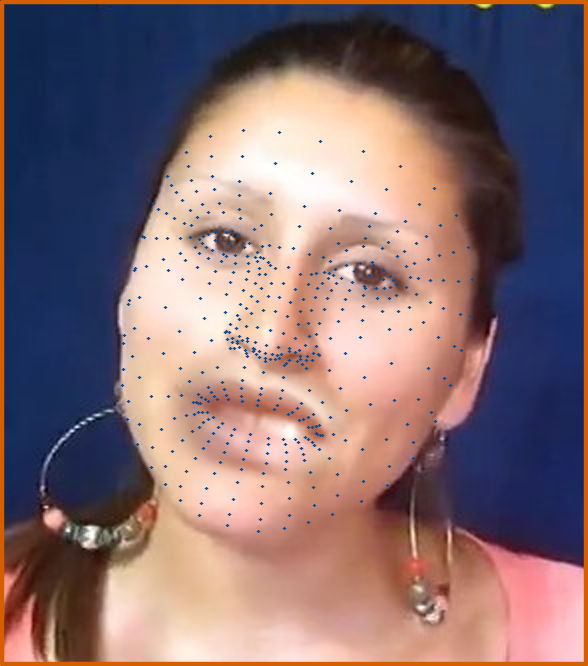
\includegraphics[width=1.0cm]{img/detect.png}};
\node[body] at ([yshift=-1.62cm]s2.north) {MediaPipe,\\[-1pt]478 landmarks;\\[-1pt]crop + 35\,\% per side};

\stg{net}{s3}{5.3}{\ya}{3.5}{\ha}{Detector}
\node[thumb] (ov) at ([xshift=-0.7cm,yshift=-0.97cm]s3.north) {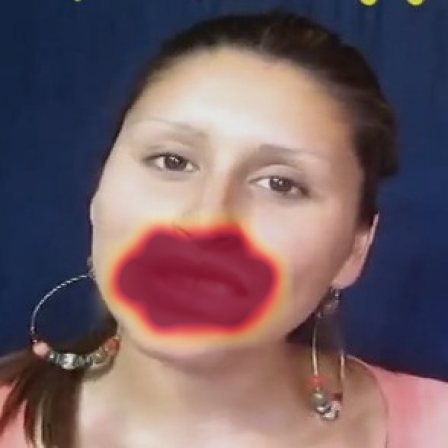
\includegraphics[width=1.0cm]{img/ev_overlay.png}};
\node[anchor=west, font=\smallfont, align=left, inner sep=0pt] at ([xshift=0.15cm]ov.east) {$z_f$,\, $z_b$\\[-0.5pt]4 operations\\[-0.5pt]\shp{16×16} map};
\node[body] at ([yshift=-1.62cm]s3.north) {CLIP ViT-L/14 + LoRA;\\[-1pt]decision: $P(\text{fake})=\sigma(z_f)$};

\stg{code}{s4}{9.35}{\ya}{3.4}{\ha}{Part mapping}
\node[thumb] at ([yshift=-0.97cm]s4.north) {
\includegraphics[width=1.0cm]{img/masks.png}};
\node[body] at ([yshift=-1.62cm]s4.north) {masks: eyes, nose, mouth,\\[-1pt]skin, contour; name the\\[-1pt]highest mean evidence;\\[-1pt]whole face if eyes, nose,\\[-1pt]mouth all $\geq$\,0.5};

\stg{io}{s5}{13.3}{\ya}{4.75}{\ha}{Structured record}
\node[anchor=north west, align=left, inner sep=0pt, font=\fontsize{5.6}{7.0}\selectfont\ttfamily] at ([xshift=0.22cm,yshift=-0.48cm]s5.north west)
  {decision: fake\\
   P: real 0.00, fake 1.00, filter 0.00\\
   ops: eye 0.05, slim 0.01,\\
   \ \ \ \ \ whiten 0.18, smooth 0.15\\
   evidence: mouth 0.99, nose 0.41,\\
   \ \ \ skin 0.28, contour 0.04, eyes 0.00\\
   named part: mouth};
\foreach \a/\b in {s1/s2,s2/s3,s3/s4,s4/s5}{\draw[flow] (\a.east) -- (\b.west);}

\node[badge=plum, anchor=south] (bdg1) at ($(s3.north east)!0.5!(s4.north west)+(0,0.13)$)
  {validated: restoring the named part removes 93.5--94.0\,\% of detections (ceiling 93.6--94.1\,\%)};
\draw[plum, densely dashed] (bdg1.south) -- ++(0,-0.13);

% ================================================================ row 2: language layer
\def\yb{1.0} \def\hb{3.25}
\stg{code}{s6}{0}{\yb}{3.0}{\hb}{Fact list (code)}
\node[anchor=north west, align=left, inner sep=0pt, font=\fontsize{5.8}{6.9}\selectfont, text width=2.75cm] at ([xshift=0.13cm,yshift=-0.45cm]s6.north west)
  {\textbf{facts}, no numbers:\\
   \textcolor{muted}{decision is fake; the evidence is concentrated on the mouth}\\[3pt]
   \textbf{must not say:}\\
   \textcolor{muted}{real or beautified; any part other than the mouth; any number; certainty or calibration}};

\stg{llm}{s7}{3.35}{\yb}{3.2}{\hb}{LLM wording}
\node[body] at ([yshift=-0.45cm]s7.north) {Qwen2.5-7B-Instruct;\\[-1pt]no image, no decision,\\[-1pt]no numbers};
\node[draw=amber!60, fill=white, rounded corners=1pt, anchor=north, font=\fontsize{5.8}{6.9}\selectfont, align=left, text width=2.85cm, inner sep=2pt]
  at ([yshift=-1.35cm]s7.north) {The model's decision is fake. The evidence is concentrated on the mouth.};

\stg{code}{s8}{6.9}{\yb}{3.6}{\hb}{Code adds numbers}
\node[body] at ([yshift=-0.45cm]s8.north) {decision score in parentheses,\\[-1pt]fixed calibration sentence};
\node[draw=okc!60, fill=white, rounded corners=1pt, anchor=north, font=\fontsize{5.8}{6.9}\selectfont, align=left, text width=3.25cm, inner sep=2pt]
  at ([yshift=-1.0cm]s8.north) {The model's decision is fake \num{(decision score 1.00)}. The evidence is concentrated on the mouth. \num{The score is the model's raw output, not a calibrated probability, and a high score does not mean the decision is correct.}};

\stg{chk}{s9}{10.85}{\yb}{4.2}{\hb}{Automatic checks}
\node[anchor=north west, align=left, inner sep=0pt, font=\fontsize{5.8}{7.1}\selectfont] at ([xshift=0.15cm,yshift=-0.47cm]s9.north west)
  {1\; decision\\ 2\; region\\ 3\; operations\\ 4\; numbers in record\\ 5\; banned phrases\\ 6\; length};
\node[anchor=north west, align=left, inner sep=0pt, font=\fontsize{5.8}{7.1}\selectfont] at ([xshift=2.2cm,yshift=-0.47cm]s9.north west)
  {7\; score vs threshold\\ 8\; certainty words\\ 9\; score on a part\\ 10\; no LLM numbers\\ 11\; all facts present};
\node[anchor=south, note, align=center, inner sep=1pt] at ([yshift=3pt]s9.south) {11 rules, applied to every text\\[-1pt]before display (Appendix A)};

\stg{io}{s10}{15.5}{\yb}{2.6}{\hb}{Output}
\node[draw=errc, fill=fFall, rounded corners=4pt, font=\smallfont\bfseries, text=errc, inner xsep=4pt, inner ysep=1.5pt] (chip)
  at ([yshift=-0.58cm]s10.north) {fake\; \textmd{\shp{1.00}}};
\node[thumb] at ([yshift=-1.4cm]s10.north) {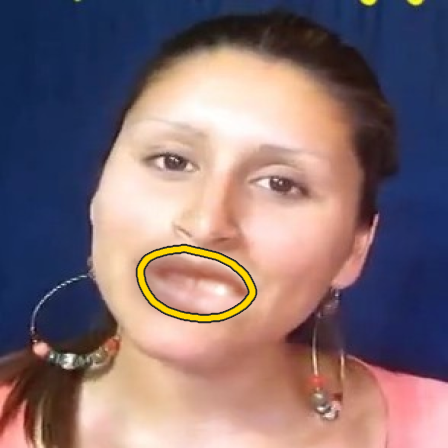
\includegraphics[width=1.0cm]{img/out_contour.png}};
\node[body] at ([yshift=-2.02cm]s10.north) {decision chip,\\[-1pt]part on the crop,\\[-1pt]checked text};
\foreach \a/\b in {s6/s7,s7/s8,s8/s9}{\draw[flow] (\a.east) -- (\b.west);}
\draw[okflow] (s9.east) -- node[above, font=\smallfont\bfseries, text=okc, inner sep=1pt]{pass} (s10.west);

% record -> fact list
\draw[flow] (s5.south) -- (s5.south |- 0,1.47) -| (s6.north);
\node[anchor=south, note, inner sep=0.8pt] at (9.0,1.47) {every word shown to the user is derived from the record};
\node[badge=plum, anchor=south] (bdg2) at ([yshift=0.07cm]s7.north) {blind test: VLM region text matched 50.6--59.0\,\%, chance 50};

% ================================================================ fallback
\node[llm, anchor=north, minimum width=3.4cm, minimum height=0.55cm, font=\smallfont] (re) at ([xshift=-0.3cm,yshift=-0.42cm]s9.south)
  {\textbf{rewrite once}\; \textcolor{muted}{(sampled, checked again)}};
\node[fall, anchor=north, minimum width=2.6cm, minimum height=0.55cm, font=\smallfont] (tpl) at ([yshift=-0.42cm]s10.south)
  {\textbf{code template}};
\draw[errflow] (re.north -| s9.south) ++(0,0.42) -- node[left, font=\smallfont\bfseries, text=errc, inner sep=2pt]{fail} (re.north -| s9.south);
\draw[errflow] (re.east) -- (tpl.west);
\node[font=\smallfont\bfseries, text=errc, anchor=north, inner sep=1pt] at ($(re.south east)!0.5!(tpl.south west)$) {fail};
\draw[okflow] ([xshift=-0.25cm]re.north east) |- (15.75,-2.42) -- (15.75,0 |- s10.south);
\node[font=\smallfont\bfseries, text=okc, anchor=west, inner sep=1pt] at (15.78,-2.33) {pass};
\draw[errflow] (tpl.north) -- (tpl.north |- s10.south);
\end{tikzpicture}
\end{document}
